%%%%%%%%%%%%%%%%%%%%%%%%%%%%%%%%%%%%%%%%%%%%%%%%%%%%%%%%%%%%%%%%%%%%%%%
% BAB 3
%%%%%%%%%%%%%%%%%%%%%%%%%%%%%%%%%%%%%%%%%%%%%%%%%%%%%%%%%%%%%%%%%%%%%%%

\mychapter{5}{BAB 5 HASIL DAN PEMBAHASAN}

\section{Hasil}

\subsection{Analisis Kondisi dan Kebutuhan Sistem}

Pada awal pelaksanaan PKL, pengembangan aplikasi SIPANTAU telah berada pada tahap pengembangan dengan beberapa komponen awal yang telah tersedia. Komponen tersebut menjadi kondisi awal yang digunakan sebagai dasar untuk memahami tujuan, mekanisme kerja, serta kebutuhan pengembangan sistem. Pada tahap ini, \textit{frontend} aplikasi telah tersedia dan digunakan untuk menampilkan antarmuka sistem dengan data \textit{dummy}. Selain itu, telah tersedia rancangan awal basis data yang menggambarkan entitas dan hubungan data yang dibutuhkan oleh aplikasi secara umum. Framework Laravel juga telah ditentukan sebagai teknologi yang digunakan untuk mengembangkan sisi \textit{backend} aplikasi.

Berdasarkan kondisi awal tersebut, aplikasi SIPANTAU dirancang untuk mendukung pengelolaan data komoditas dan harga pada pasar serta menyediakan fungsi prediksi harga komoditas untuk tiga hari ke depan. Proses penggunaan aplikasi melibatkan pengguna sebagai pihak yang berinteraksi dengan sistem melalui \textit{frontend}, sedangkan pengolahan data dilakukan melalui \textit{backend} yang terhubung dengan basis data. Fungsi prediksi membutuhkan data historis yang tersimpan pada basis data untuk kemudian diproses oleh layanan model prediksi. Selain fungsi pengelolaan data dan prediksi, sistem juga membutuhkan mekanisme \textit{authentication} dan \textit{authorization} untuk mengatur akses pengguna berdasarkan peran yang dimiliki.

Kondisi awal aplikasi dan tujuan sistem tersebut kemudian dianalisis untuk menentukan kebutuhan yang perlu dipenuhi pada pengembangan \textit{backend}. Analisis dilakukan dengan mengidentifikasi fungsi utama yang diperlukan agar \textit{frontend} yang telah tersedia dapat terhubung dengan data aktual melalui API, pengguna dapat mengakses sistem sesuai dengan hak aksesnya, serta proses prediksi dapat dijalankan melalui layanan model yang telah tersedia. Hasil identifikasi tersebut mencakup kebutuhan pengelolaan data aplikasi, kebutuhan pengelolaan pengguna dan hak akses, kebutuhan penyediaan API, serta kebutuhan integrasi dengan layanan model prediksi.

Kondisi awal \textit{frontend} yang menggunakan data \textit{dummy} digunakan sebagai salah satu acuan untuk mengidentifikasi data dan fungsi yang perlu disediakan oleh \textit{backend}. Sementara itu, rancangan awal basis data digunakan sebagai acuan awal dalam memahami struktur data yang dibutuhkan oleh aplikasi. Kedua komponen tersebut kemudian dianalisis kembali berdasarkan kebutuhan sistem sehingga dapat ditentukan fungsi dan interaksi yang perlu didukung oleh \textit{backend}. Beberapa gambaran kondisi awal \textit{frontend} dapat dilihat pada Gambar \ref{fig:fe-awal-lp}, \ref{fig:fe-awal-input}, dan \ref{fig:fe-awal-prediksi}, sedangkan rancangan awal basis data dapat dilihat pada Gambar \ref{fig:db-awal}.

\begin{figure}[ht]
    \centering
    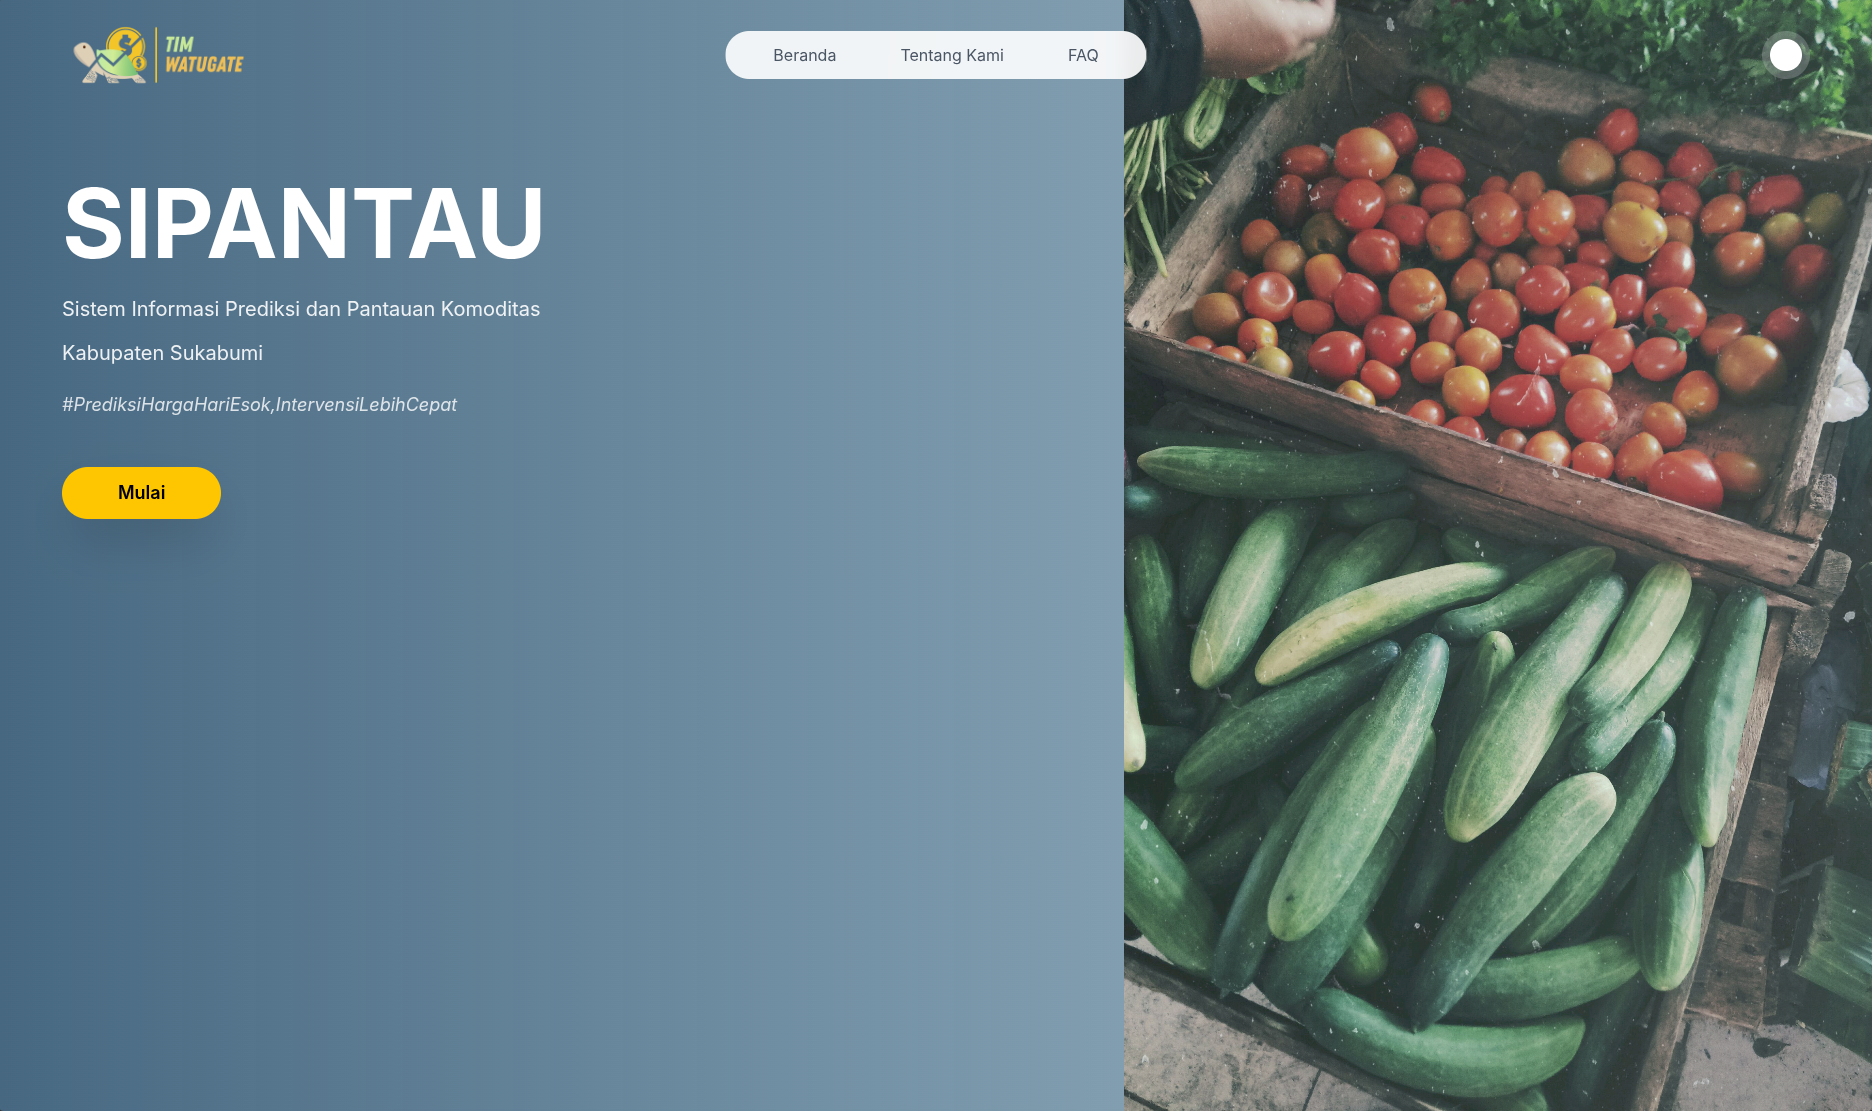
\includegraphics[width=0.75\textwidth]{img/fe-awal-lp.png}
    \caption{Kondisi awal frontend \textit{landing page} SIPANTAU}
    \label{fig:fe-awal-lp}
\end{figure}

\begin{figure}[ht]
    \centering
    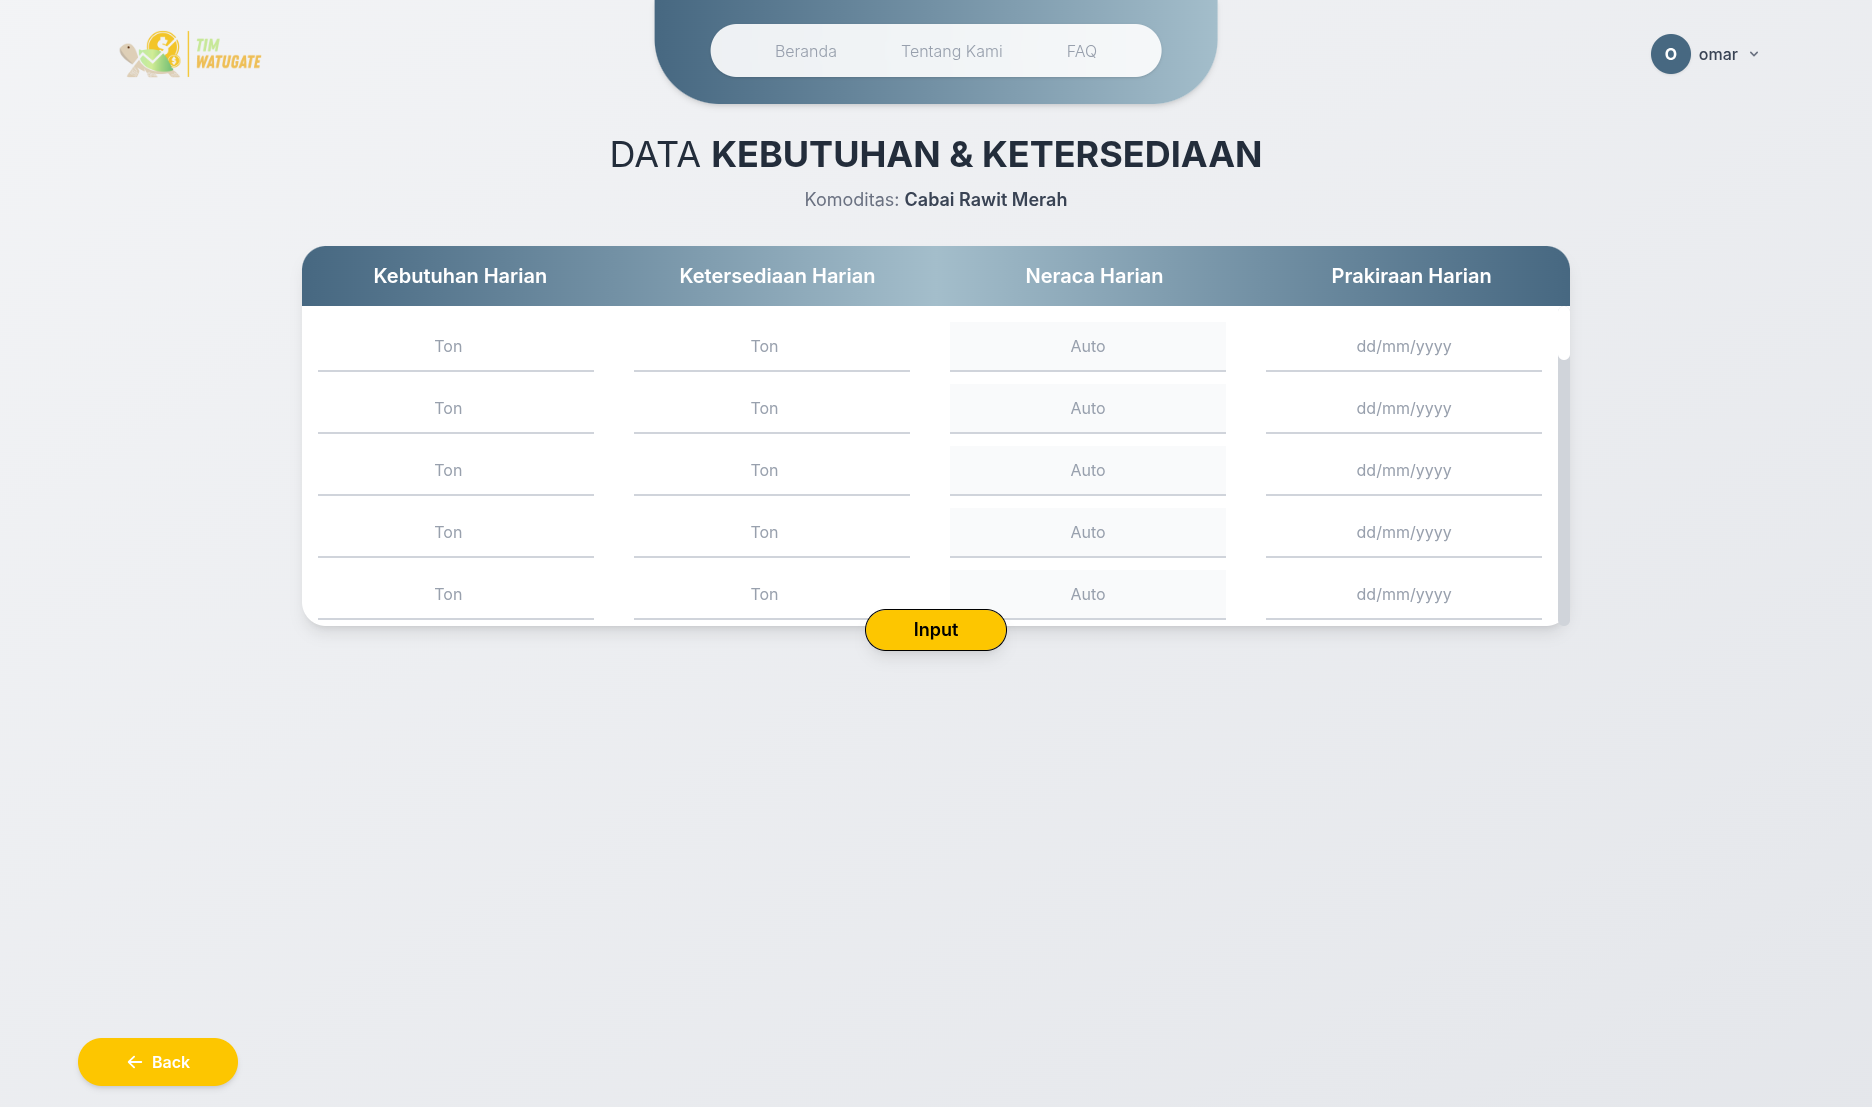
\includegraphics[width=0.75\textwidth]{img/fe-awal-input.png}
    \caption{Kondisi awal frontend halaman input data SIPANTAU}
    \label{fig:fe-awal-input}
\end{figure}

\begin{figure}[ht]
    \centering
    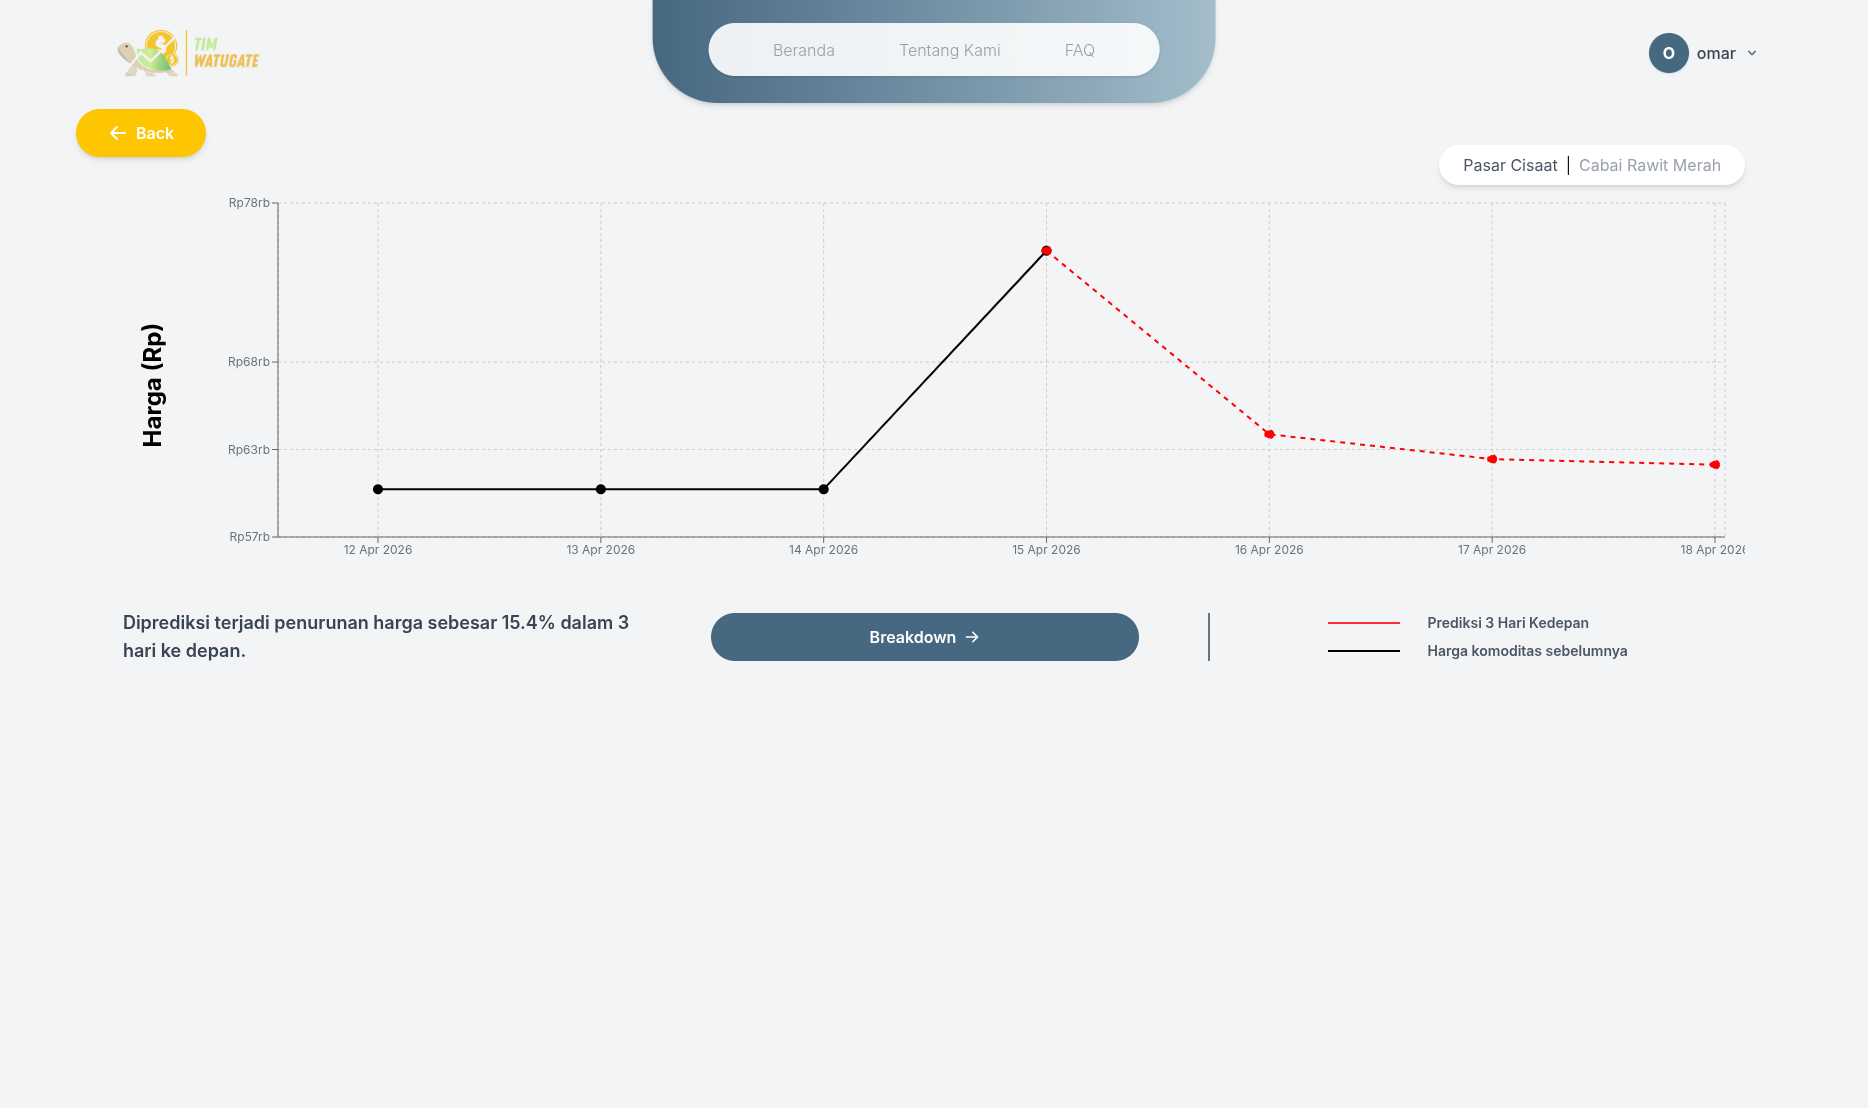
\includegraphics[width=0.75\textwidth]{img/fe-awal-prediksi.png}
    \caption{Kondisi awal frontend halaman prediksi SIPANTAU}
    \label{fig:fe-awal-prediksi}
\end{figure}

\begin{figure}[ht]
    \centering
    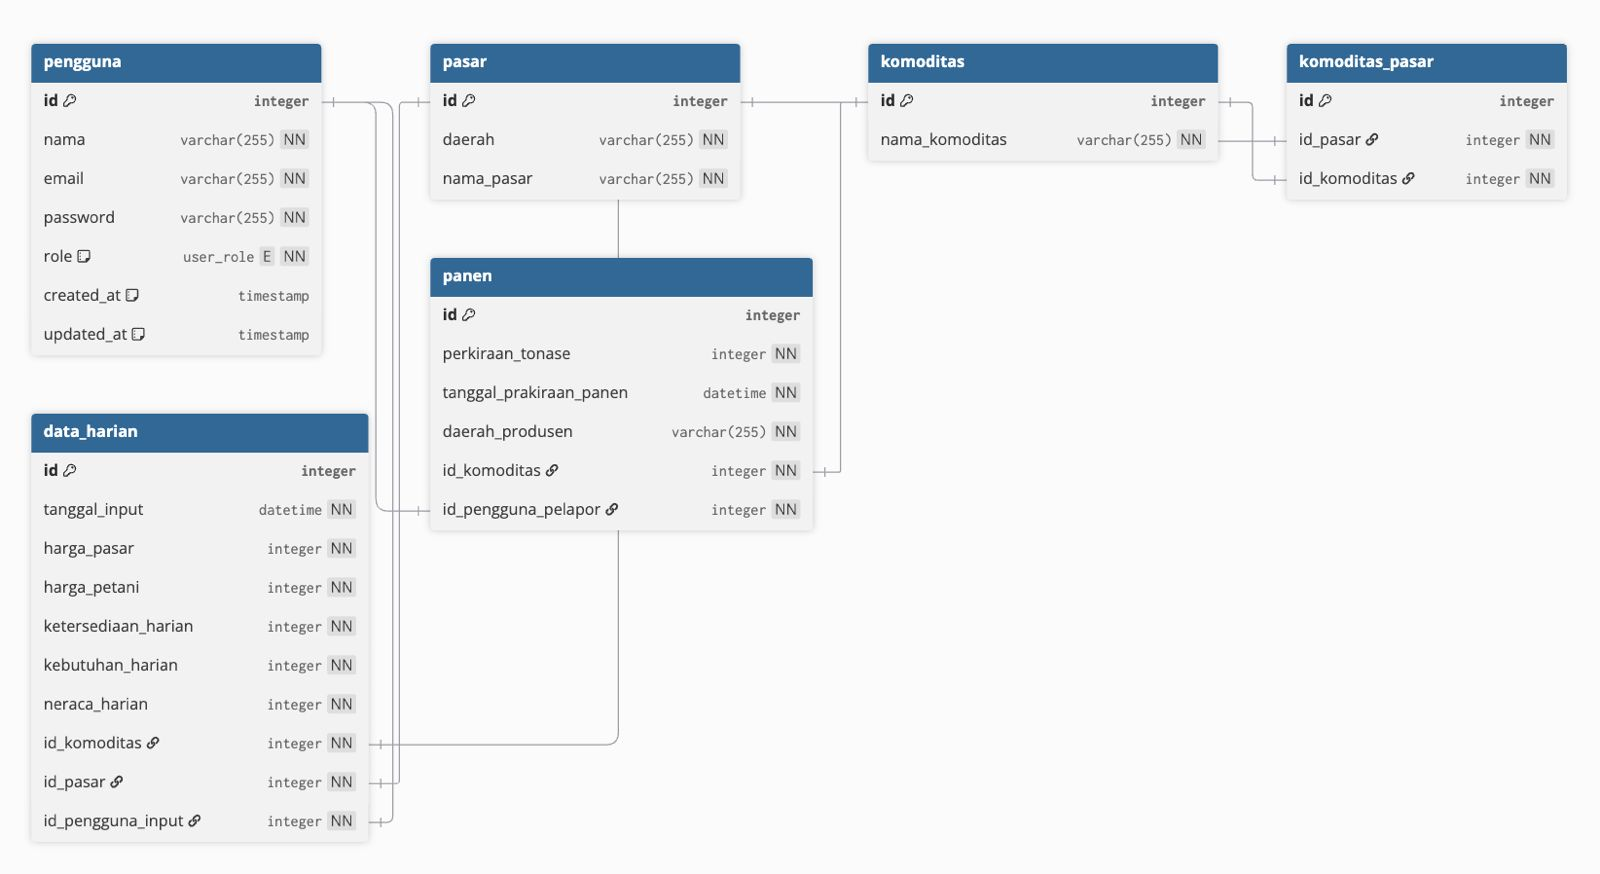
\includegraphics[width=0.75\textwidth]{img/db-awal.jpeg}
    \caption{Rancangan awal basis data SIPANTAU}
    \label{fig:db-awal}
\end{figure}

\FloatBarrier

Berdasarkan hasil identifikasi terhadap kondisi awal dan tujuan pengembangan SIPANTAU, diperoleh sejumlah kebutuhan fungsional yang harus dipenuhi oleh sistem. Kebutuhan tersebut mencakup mekanisme autentikasi dan otorisasi pengguna, pengelolaan data komoditas, penyediaan data melalui API, serta penyediaan fungsi prediksi harga komoditas. Kebutuhan fungsional yang diperoleh dari hasil analisis disajikan pada Tabel \ref{tab:kebutuhan-fungsional}.

\begin{longtable}{|c|c|p{5.0cm}|p{5.0cm}|}
    \caption{Kebutuhan fungsional SIPANTAU}
    \label{tab:kebutuhan-fungsional} \\
    \hline
    \textbf{No.} &
    \textbf{Kode} &
    \textbf{Kebutuhan Fungsional} &
    \textbf{Keterangan} \\
    \hline
    \endfirsthead

    \hline
    \textbf{No.} &
    \textbf{Kode} &
    \textbf{Kebutuhan Fungsional} &
    \textbf{Keterangan} \\
    \hline
    \endhead

    1 &
    KF-01 &
    Sistem dapat melakukan autentikasi pengguna. &
    Sistem melakukan verifikasi identitas pengguna sebelum pengguna mengakses fungsi yang memerlukan autentikasi. \\
    \hline

    2 &
    KF-02 &
    Sistem dapat melakukan otorisasi pengguna berdasarkan peran. &
    Sistem mengatur hak akses pengguna terhadap fungsi aplikasi berdasarkan peran yang dimiliki. \\
    \hline

    3 &
    KF-03 &
    Sistem dapat menerima dan mengelola data kebutuhan dan ketersediaan komoditas. &
    Pengguna yang memiliki hak akses dapat memasukkan dan mengelola data kebutuhan serta ketersediaan komoditas. \\
    \hline

    4 &
    KF-04 &
    Sistem dapat menerima dan mengelola data panen komoditas. &
    Pengguna yang memiliki hak akses dapat memasukkan dan mengelola data hasil panen komoditas. \\
    \hline

    5 &
    KF-05 &
    Sistem dapat menerima dan mengelola data harga petani. &
    Pengguna yang memiliki hak akses dapat memasukkan dan mengelola data harga komoditas pada tingkat petani. \\
    \hline

    6 &
    KF-06 &
    Sistem dapat menerima dan mengelola data harga pasar. &
    Pengguna yang memiliki hak akses dapat memasukkan dan mengelola data harga komoditas pada pasar. \\
    \hline

    7 &
    KF-07 &
    Sistem dapat menyediakan data melalui API. &
    Sistem menyediakan API yang memungkinkan data digunakan oleh komponen aplikasi yang membutuhkan. \\
    \hline

    8 &
    KF-08 &
    Sistem dapat menampilkan hasil prediksi harga komoditas untuk tiga hari ke depan. &
    Sistem menggunakan data historis yang diperlukan untuk memperoleh hasil prediksi harga melalui layanan model prediksi. \\
    \hline

\end{longtable}

Selain kebutuhan fungsional, hasil analisis juga mengidentifikasi beberapa kebutuhan non-fungsional yang berkaitan dengan batasan teknologi, keamanan, dan lingkungan operasional sistem. Pada awal pengembangan, teknologi yang digunakan pada \textit{frontend} telah ditetapkan menggunakan Next.js, sedangkan \textit{backend} ditetapkan untuk dikembangkan menggunakan Laravel. Selain itu, aspek keamanan dan penggunaan VPS yang telah disediakan juga menjadi batasan pengembangan sistem. Berdasarkan proses analisis dan perancangan, kebutuhan non-fungsional tersebut menjadi acuan dalam menentukan teknologi dan mekanisme implementasi aplikasi. Rincian kebutuhan non-fungsional SIPANTAU disajikan pada Tabel \ref{tab:kebutuhan-nonfungsional}.

\begin{longtable}{|c|c|p{5.0cm}|p{5.0cm}|}
    \caption{Kebutuhan non-fungsional SIPANTAU}
    \label{tab:kebutuhan-nonfungsional} \\
    \hline
    \textbf{No.} &
    \textbf{Kode} &
    \textbf{Kebutuhan Non-Fungsional} &
    \textbf{Keterangan} \\
    \hline
    \endfirsthead

    \hline
    \textbf{No.} &
    \textbf{Kode} &
    \textbf{Kebutuhan Non-Fungsional} &
    \textbf{Keterangan} \\
    \hline
    \endhead

    1 &
    KNF-01 &
    Sistem harus menerapkan keamanan pada aplikasi. &
    Sistem harus menerapkan mekanisme keamanan untuk melindungi akses dan komunikasi pada aplikasi. \\
    \hline

    2 &
    KNF-02 &
    Sistem harus dapat dideploy pada VPS yang telah disediakan. &
    Aplikasi harus dapat dijalankan pada lingkungan VPS yang disediakan sebagai lingkungan \textit{deployment}. \\
    \hline

    3 &
    KNF-03 &
    Pengembangan backend harus dapat diintegrasikan dengan frontend berbasis Next.js. &
    Backend yang dikembangkan harus menyediakan mekanisme komunikasi yang sesuai agar dapat digunakan oleh frontend yang telah dikembangkan menggunakan Next.js. \\
    \hline

    4 &
    KNF-04 &
    Backend harus dikembangkan menggunakan Laravel. &
    Pengembangan backend harus menggunakan framework Laravel sesuai dengan teknologi yang telah ditetapkan pada awal proyek. \\
    \hline

    5 &
    KNF-05 &
    Sistem harus menjaga konsistensi data. &
    Data yang disimpan dan diperbarui melalui aplikasi harus tetap konsisten dengan kondisi data pada basis data. \\
    \hline

\end{longtable}

Berdasarkan kebutuhan fungsional dan non-fungsional yang telah diidentifikasi, selanjutnya sistem dimodelkan untuk menggambarkan hubungan antara pengguna dengan fungsi yang tersedia pada SIPANTAU. Pemodelan tersebut menggambarkan aktor yang terlibat dalam sistem serta fungsi yang dapat dijalankan oleh masing-masing aktor sesuai dengan tanggung jawabnya. SIPANTAU memiliki lima aktor utama, yaitu Dinas Perdagangan, Dinas Ketahanan Pangan, Dinas Pertanian, Tim Pengendalian Inflasi Daerah (TPID), dan Admin.

Dinas Perdagangan menginput data harga pasar, sedangkan Dinas Ketahanan Pangan menginput data kebutuhan dan ketersediaan komoditas. Dinas Pertanian menginput data panen dan data harga komoditas pada tingkat petani. Ketiga perangkat daerah tersebut memperbarui data secara berkala agar sistem memiliki data yang mutakhir untuk mendukung proses prediksi harga komoditas.TPID menggunakan SIPANTAU untuk melihat hasil prediksi harga komoditas,sedangkan Admin memiliki akses terhadap seluruh fungsi sistem, termasuk melakukan registrasi akun pengguna.

Setiap aktor melakukan autentikasi sebelum mengakses fungsi yang memerlukan akses pengguna. Sistem menerapkan pembatasan hak akses berdasarkan peran pengguna sehingga setiap aktor hanya dapat menjalankan fungsi yang sesuai dengan kewenangannya. Hubungan antara aktor dan fungsi yang tersedia pada SIPANTAU ditunjukkan pada Gambar \ref{fig:use-case-sipantau}.

\begin{figure}[ht]
    \centering
    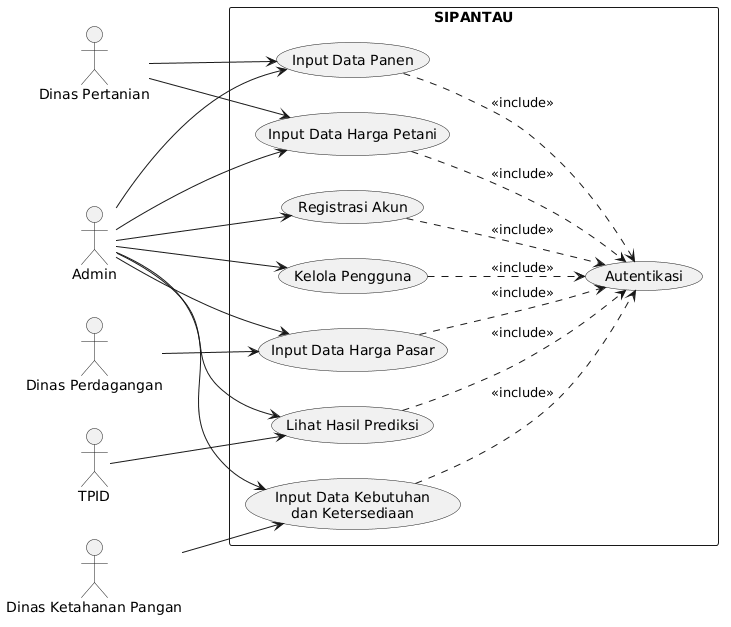
\includegraphics[width=0.75\textwidth]{img/use-case-sipantau.png}
    \caption{Use Case Diagram SIPANTAU}
    \label{fig:use-case-sipantau}
\end{figure}

Gambar \ref{fig:use-case-sipantau} menunjukkan pembagian fungsi SIPANTAU berdasarkan peran masing-masing aktor. Dinas Perdagangan mengelola data harga pasar, Dinas Ketahanan Pangan mengelola data kebutuhan dan ketersediaan, sedangkan Dinas Pertanian mengelola data panen dan harga petani. TPID melihat hasil prediksi harga komoditas, sedangkan Admin mengakses seluruh fungsi yang t   ersedia dan melakukan registrasi akun pengguna. Setiap aktor melakukan autentikasi sebelum mengakses fungsi sistem sesuai dengan hak akses yang dimilikinya.

Setelah hubungan antara aktor dan fungsi sistem ditentukan melalui Use Case Diagram, analisis dilanjutkan dengan menggambarkan alur aktivitas pada fungsi utama SIPANTAU. Activity Diagram menunjukkan urutan aktivitas yang dilakukan oleh pengguna dan komponen sistem dalam menjalankan setiap fungsi. Diagram tersebut mencakup proses autentikasi, registrasi akun, pengelolaan data, dan prediksi harga.

\begin{center}
    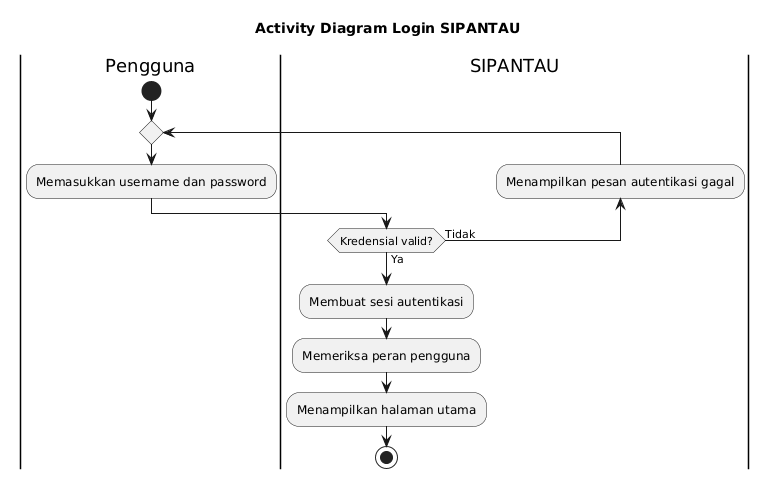
\includegraphics[width=0.8\textwidth]{img/ad-login.png}
    \captionof{figure}{Activity Diagram Autentikasi SIPANTAU}
    \label{fig:activity-login}
\end{center}

Activity Diagram autentikasi pada Gambar \ref{fig:activity-login} menggambarkan proses pengguna saat masuk ke SIPANTAU. Pengguna memasukkan username dan password, kemudian SIPANTAU memverifikasi kredensial tersebut. Sistem menampilkan pesan autentikasi gagal apabila kredensial tidak valid dan mengembalikan alur ke proses pengisian kredensial. Apabila kredensial valid, sistem membuat sesi autentikasi dan memeriksa peran pengguna sebelum menampilkan halaman utama. Alur tersebut memastikan bahwa pengguna telah terautentikasi sebelum mengakses fungsi yang tersedia pada sistem.

\begin{center}
    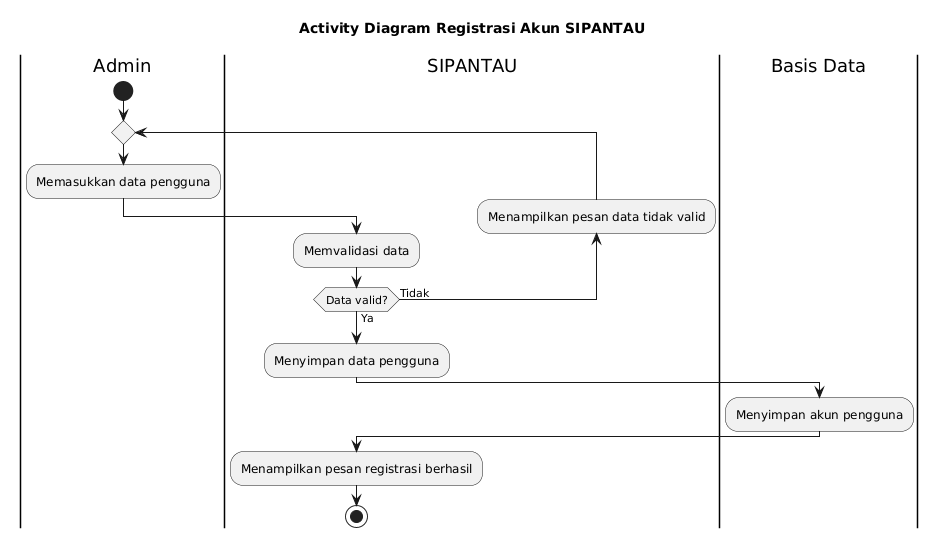
\includegraphics[width=0.8\textwidth]{img/ad-registrasi.png}
    \captionof{figure}{Activity Diagram Registrasi Akun SIPANTAU}
    \label{fig:activity-registrasi}
\end{center}

Activity Diagram registrasi akun pada Gambar \ref{fig:activity-registrasi} menggambarkan proses Admin dalam menambahkan akun pengguna ke SIPANTAU. Admin memasukkan data pengguna dan menentukan peran pengguna, kemudian SIPANTAU memvalidasi data tersebut sebelum menyimpannya. Sistem menampilkan pesan kesalahan apabila data tidak memenuhi validasi dan mengembalikan alur ke proses pengisian data. Apabila data valid, SIPANTAU menyimpan akun pengguna pada basis data dan menampilkan pesan bahwa proses registrasi berhasil.

\begin{center}
    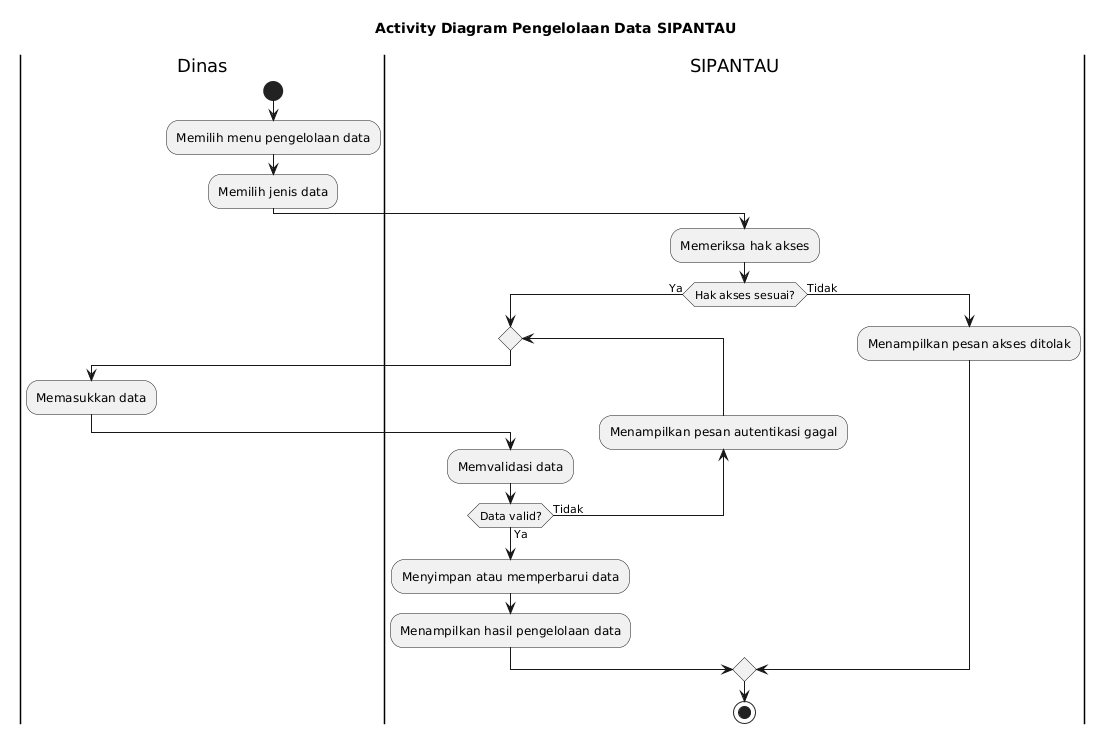
\includegraphics[width=0.8\textwidth]{img/ad-input.png}
    \captionof{figure}{Activity Diagram Pengelolaan Data SIPANTAU}
    \label{fig:activity-pengelolaan-data}
\end{center}

Activity Diagram pengelolaan data pada Gambar \ref{fig:activity-pengelolaan-data} menggambarkan proses Dinas dalam memasukkan dan mengelola data pada SIPANTAU. Dinas memilih menu dan jenis data yang sesuai dengan tanggung jawabnya, kemudian memasukkan data ke dalam sistem. SIPANTAU memeriksa hak akses pengguna sebelum memproses data dan melakukan validasi terhadap data yang dimasukkan. Sistem menampilkan pesan kesalahan apabila data tidak valid dan mengembalikan alur ke proses pengisian data. Apabila data telah memenuhi validasi, sistem menyimpan atau memperbarui data pada basis data dan menampilkan hasil pengelolaan data kepada pengguna.

\begin{center}
    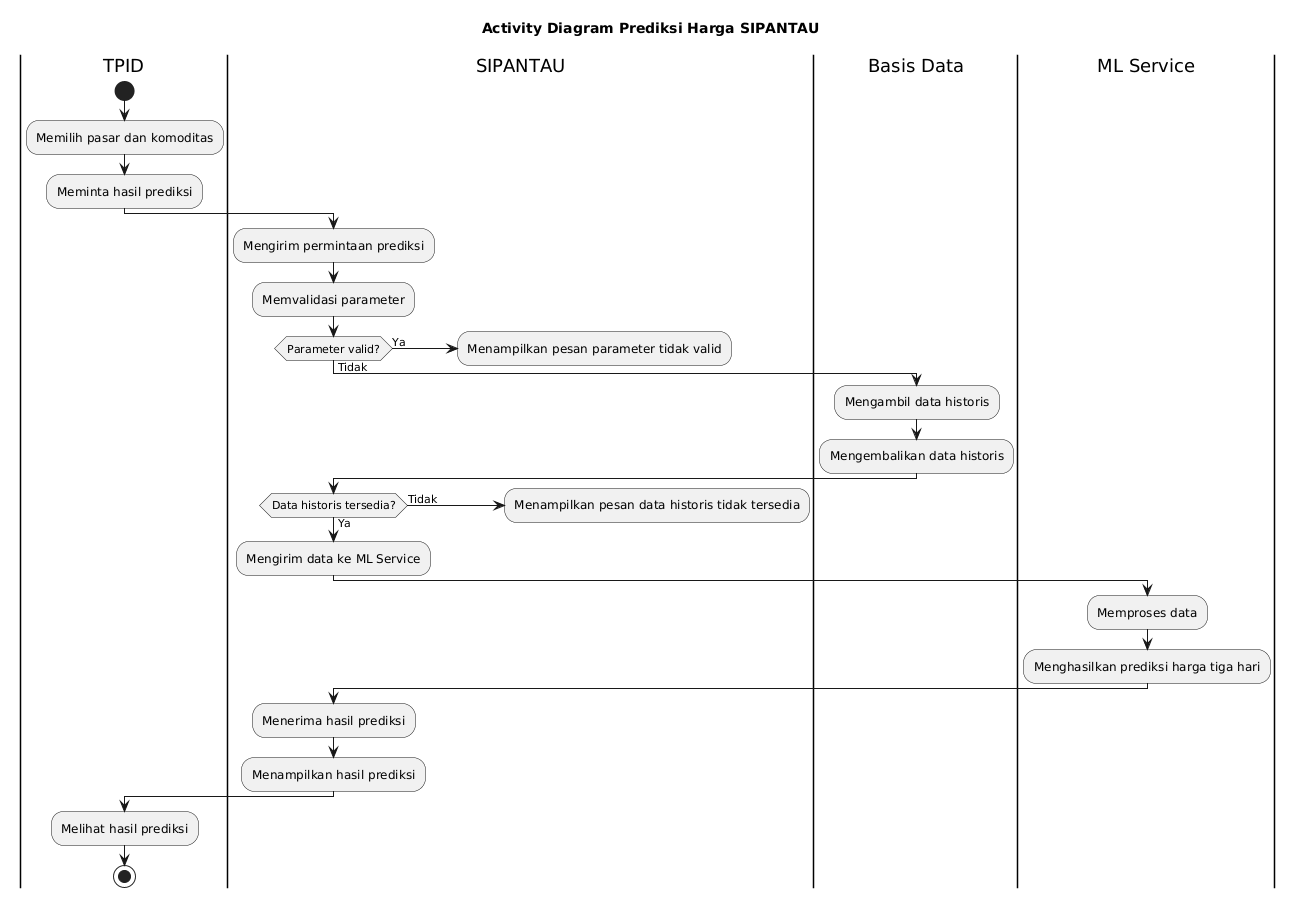
\includegraphics[width=0.8\textwidth]{img/ad-prediksi.png}
    \captionof{figure}{Activity Diagram Prediksi Harga SIPANTAU}
    \label{fig:activity-prediksi}
\end{center}

Activity Diagram prediksi harga pada Gambar \ref{fig:activity-prediksi} menggambarkan alur permintaan prediksi dari TPID hingga hasil prediksi ditampilkan. TPID memilih pasar dan komoditas, kemudian frontend mengirimkan permintaan prediksi kepada SIPANTAU. SIPANTAU memvalidasi parameter yang dikirimkan dan menampilkan pesan kesalahan pada frontend apabila parameter tidak valid. Setelah parameter valid, sistem mengambil data historis dari basis data dan memeriksa ketersediaan data tersebut.

Keempat Activity Diagram tersebut memperlihatkan alur utama yang perlu didukung oleh SIPANTAU berdasarkan kebutuhan yang telah diidentifikasi. Alur autentikasi memastikan pengguna dapat mengakses sistem sesuai dengan identitas dan perannya, sedangkan alur registrasi akun mendukung Admin dalam menyediakan akun bagi pengguna. Alur pengelolaan data mendukung pembaruan data komoditas oleh Dinas, sementara alur prediksi menghubungkan data historis dengan layanan model prediksi untuk menghasilkan prediksi harga. Hasil analisis tersebut menjadi dasar dalam menentukan rancangan basis data, arsitektur backend, mekanisme hak akses, integrasi layanan model prediksi, dan deployment aplikasi.

\subsection{Perancangan, Implementasi, dan Pengujian Backend dan Basis Data}

Bagian ini membahas hasil perancangan, implementasi, dan pengujian backend serta basis data SIPANTAU. Perancangan mencakup struktur basis data, arsitektur backend, dan penyediaan API untuk mendukung fungsi sistem yang telah ditetapkan. Implementasi kemudian merealisasikan rancangan tersebut menggunakan teknologi yang telah ditentukan, sedangkan pengujian dilakukan untuk memastikan fungsi backend dan basis data berjalan sesuai kebutuhan sistem.

\subsubsection{Perancangan}

Perancangan backend dan basis data dilakukan berdasarkan kebutuhan fungsional dan non-fungsional yang telah diidentifikasi pada tahap analisis. Perancangan tersebut mencakup struktur basis data, arsitektur backend, dan rancangan API yang digunakan untuk menyediakan dan mengelola data SIPANTAU.

Perancangan basis data menentukan struktur data dan hubungan antarentitas yang digunakan oleh SIPANTAU. Rancangan tersebut mencakup entitas pengguna, pasar, komoditas, harga pasar harian, harga petani harian, ketersediaan harian, dan panen. Hasil perancangan basis data SIPANTAU ditunjukkan pada Gambar \ref{fig:erd-sipantau}.

\begin{center}
    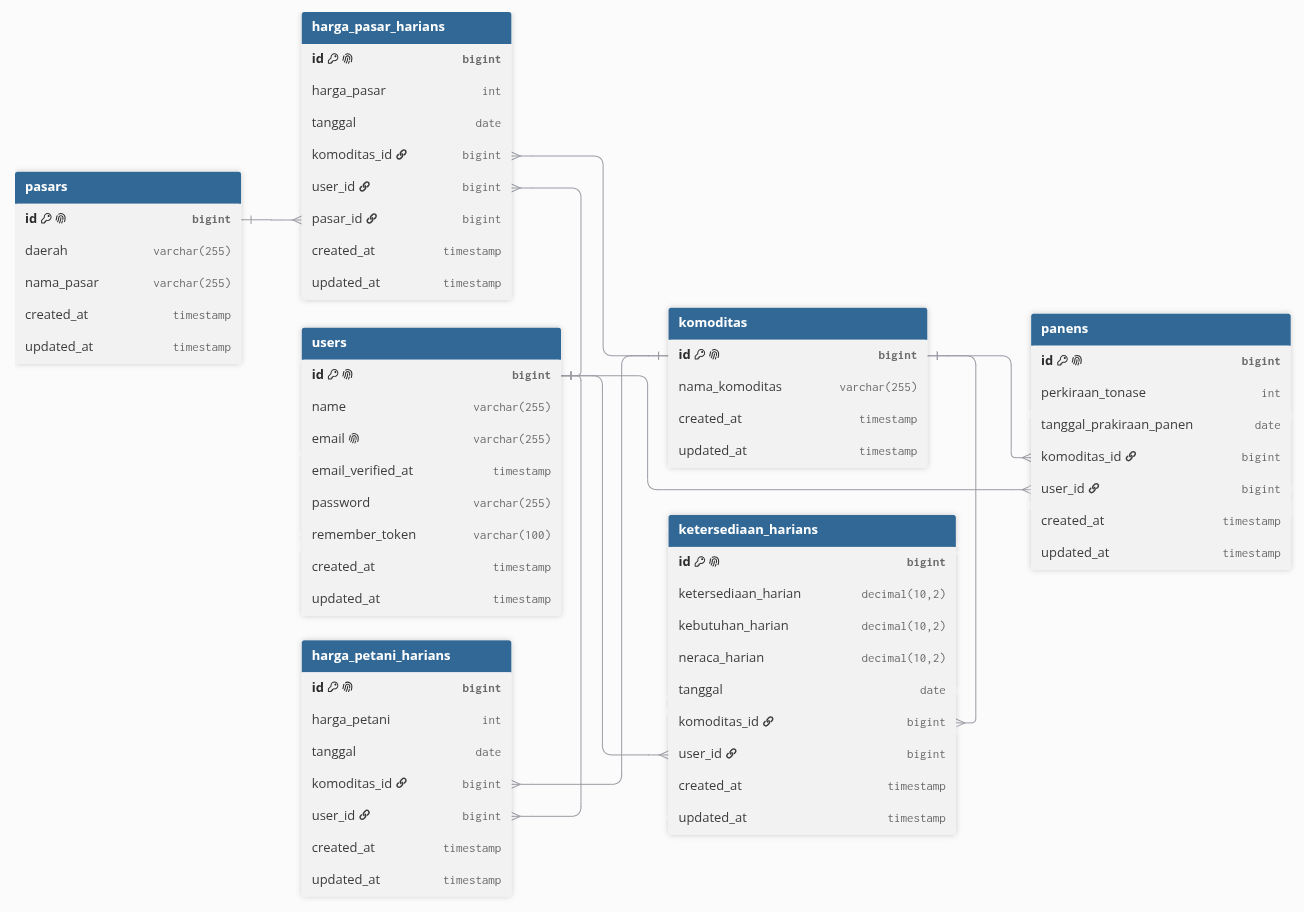
\includegraphics[width=\textwidth]{img/erd-sipantau.png}
    \captionof{figure}{Entity Relationship Diagram SIPANTAU}
    \label{fig:erd-sipantau}
\end{center}

Struktur basis data pada Gambar \ref{fig:erd-sipantau} menghubungkan data operasional dengan data referensi yang digunakan oleh SIPANTAU. Entitas \textit{komoditas} menjadi acuan bagi data harga pasar, harga petani, ketersediaan, dan panen, sedangkan entitas \textit{pasars} menjadi acuan bagi pencatatan harga pasar. Entitas \textit{users} terhubung dengan data yang dimasukkan oleh pengguna sehingga sistem dapat mencatat pengguna yang melakukan pengelolaan data.

\begin{longtable}{|c|p{4.1cm}|p{2.8cm}|p{2.3cm}|p{1.8cm}|}

    \caption{Relasi antartabel basis data SIPANTAU}
    \label{tab:relasi-database} \\

    \hline

    \multicolumn{1}{|c|}{\textbf{No.}} &
    \multicolumn{1}{c|}{\textbf{Tabel}} &
    \multicolumn{1}{c|}{\textbf{Kolom FK}} &
    \multicolumn{1}{c|}{
        \makecell[c]{\vspace{3pt}\textbf{Tabel}\\\textbf{Referensi}}
    } &
    \multicolumn{1}{c|}{
        \makecell[c]{\vspace{3pt}\textbf{Kolom}\\\textbf{Referensi}}
    } \\

    \hline
    \endfirsthead

    \hline

    \multicolumn{1}{|c|}{\textbf{No.}} &
    \multicolumn{1}{c|}{\textbf{Tabel}} &
    \multicolumn{1}{c|}{\textbf{Kolom FK}} &
    \multicolumn{1}{c|}{
        \makecell[c]{\vspace{3pt}\textbf{Tabel}\\\textbf{Referensi}}
    } &
    \multicolumn{1}{c|}{
        \makecell[c]{\vspace{3pt}\textbf{Kolom}\\\textbf{Referensi}}
    } \\

    \hline
    \endhead

    1 & \textit{harga\_pasar\_harians} & \textit{komoditas\_id} & \textit{komoditas} & \textit{id} \\ \hline
    2 & \textit{harga\_pasar\_harians} & \textit{user\_id} & \textit{users} & \textit{id} \\ \hline
    3 & \textit{harga\_pasar\_harians} & \textit{pasar\_id} & \textit{pasars} & \textit{id} \\ \hline
    4 & \textit{harga\_petani\_harians} & \textit{komoditas\_id} & \textit{komoditas} & \textit{id} \\ \hline
    5 & \textit{harga\_petani\_harians} & \textit{user\_id} & \textit{users} & \textit{id} \\ \hline
    6 & \textit{ketersediaan\_harians} & \textit{komoditas\_id} & \textit{komoditas} & \textit{id} \\ \hline
    7 & \textit{ketersediaan\_harians} & \textit{user\_id} & \textit{users} & \textit{id} \\ \hline
    8 & \textit{panens} & \textit{komoditas\_id} & \textit{komoditas} & \textit{id} \\ \hline
    9 & \textit{panens} & \textit{user\_id} & \textit{users} & \textit{id} \\ \hline

\end{longtable}

Tabel \ref{tab:relasi-database} menunjukkan hubungan antartabel yang digunakan dalam basis data SIPANTAU. Relasi tersebut menghubungkan data operasional dengan data pengguna dan data referensi yang diperlukan oleh sistem.

Perancangan backend selanjutnya menentukan struktur layanan yang mengelola proses bisnis SIPANTAU berdasarkan struktur basis data yang telah dirancang. Backend menggunakan Laravel untuk menerima dan memproses permintaan dari pengguna melalui frontend berbasis Next.js. Nginx digunakan sebagai API Gateway dan reverse proxy yang mengatur lalu lintas permintaan menuju layanan frontend dan backend. Backend Laravel berkomunikasi dengan basis data MySQL untuk mengelola data SIPANTAU dan berkomunikasi dengan ML Service berbasis FastAPI untuk menjalankan proses prediksi harga.

\begin{center}

    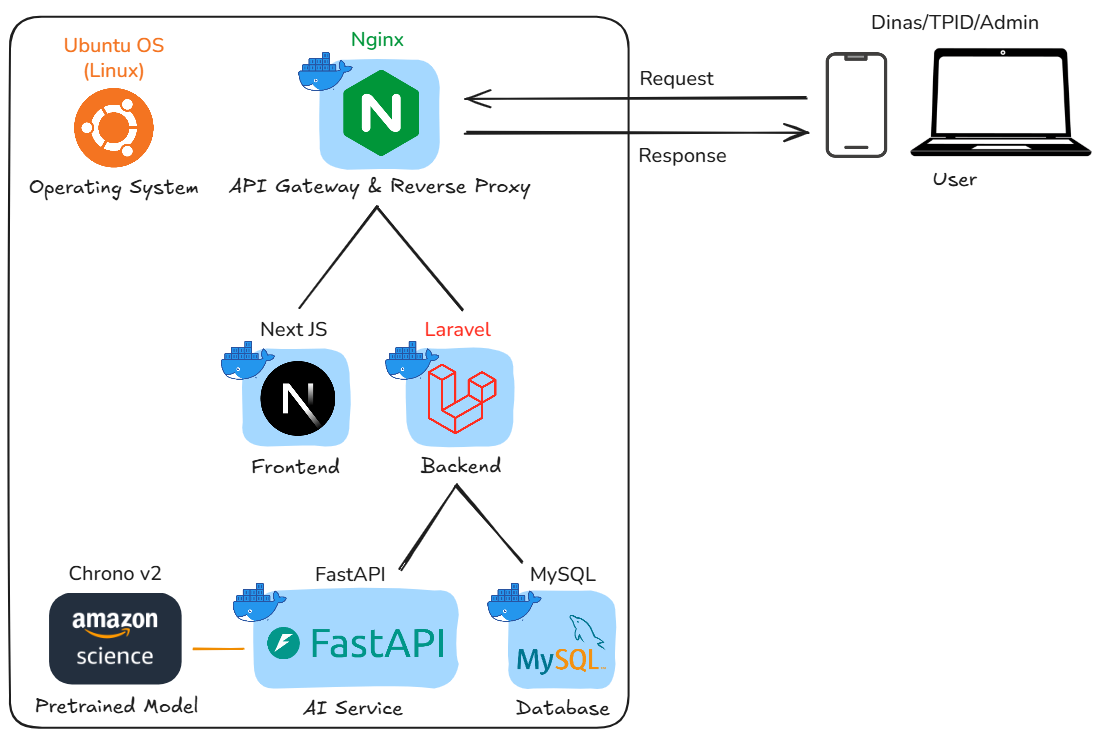
\includegraphics[width=1\textwidth]{img/arsitektur.png}

    \captionof{figure}{Arsitektur SIPANTAU}

    \label{fig:arsitektur-sipantau}

\end{center}

Arsitektur SIPANTAU pada Gambar \ref{fig:arsitektur-sipantau} menunjukkan hubungan antara komponen aplikasi yang digunakan dalam sistem. Sistem berjalan pada lingkungan Ubuntu yang menjadi sistem operasi tempat seluruh layanan aplikasi dijalankan. Nginx berperan sebagai API Gateway dan reverse proxy yang menerima permintaan dari pengguna dan meneruskannya kepada layanan yang sesuai. Frontend menggunakan Next.js untuk menyediakan antarmuka pengguna, sedangkan backend menggunakan Laravel untuk menangani proses bisnis dan menyediakan API.

Backend Laravel terhubung dengan basis data MySQL untuk menyimpan dan mengambil data yang digunakan oleh sistem. Backend juga terhubung dengan ML Service berbasis FastAPI untuk menjalankan proses prediksi harga. ML Service menggunakan model yang telah dilatih sebelumnya sebagai dasar proses prediksi. Dengan rancangan tersebut, proses pengelolaan data dan proses prediksi ditempatkan pada layanan yang terpisah sehingga masing-masing layanan dapat menjalankan tanggung jawabnya secara khusus.

Perancangan API selanjutnya menentukan endpoint yang digunakan untuk mendukung fungsi backend SIPANTAU dalam ruang lingkup pengembangan. Backend Laravel menyediakan endpoint untuk autentikasi pengguna, registrasi akun, pengelolaan data komoditas dan pasar, serta pengelolaan data ketersediaan, panen, harga pasar, dan harga petani.

\begin{longtable}{|c|c|p{3cm}|p{6.4cm}|}

    \caption{Rancangan endpoint API SIPANTAU}
    \label{tab:rancangan-api} \\

    \hline

    \textbf{No.} &
    \textbf{Method} &
    \textbf{Endpoint} &
    \textbf{Fungsi} \\

    \hline
    \endfirsthead

    \hline

    \textbf{No.} &
    \textbf{Method} &
    \textbf{Endpoint} &
    \textbf{Fungsi} \\

    \hline
    \endhead

    1 & POST & \texttt{/login} &
    Melakukan autentikasi pengguna. \\ \hline

    2 & POST & \texttt{/logout} &
    Mengakhiri sesi autentikasi pengguna. \\ \hline

    3 & GET & \texttt{/me} &
    Mengambil informasi pengguna yang sedang terautentikasi. \\ \hline

    4 & POST & \texttt{/register} &
    Mendaftarkan akun pengguna baru. \\ \hline

    5 & GET & \texttt{/komoditas} &
    Mengambil data komoditas. \\ \hline

    6 & POST & \texttt{/komoditas} &
    Menambahkan data komoditas baru. \\ \hline

    7 & GET & \texttt{/pasar} &
    Mengambil data pasar. \\ \hline

    8 & POST & \texttt{/pasar} &
    Menambahkan data pasar baru. \\ \hline

    9 & POST & \texttt{/ketersediaan} &
    Menyimpan data ketersediaan dan kebutuhan harian komoditas. \\ \hline

    10 & GET & \texttt{/ketersediaan} &
    Mengambil data ketersediaan harian. \\ \hline

    11 & POST & \texttt{/panen} &
    Menyimpan data perkiraan panen komoditas. \\ \hline

    12 & GET & \texttt{/panen} &
    Mengambil data panen. \\ \hline

    13 & POST & \texttt{/harga-pasar} &
    Menyimpan data harga pasar harian. \\ \hline

    14 & GET & \texttt{/harga-pasar} &
    Mengambil data harga pasar harian. \\ \hline

    15 & POST & \texttt{/harga-petani} &
    Menyimpan data harga petani harian. \\ \hline

    16 & GET & \texttt{/harga-petani} &
    Mengambil data harga petani harian. \\ \hline

\end{longtable}

Tabel \ref{tab:rancangan-api} menunjukkan endpoint API yang digunakan untuk mendukung pengelolaan data pada SIPANTAU. Endpoint tersebut menyediakan operasi untuk menyimpan dan mengambil data yang digunakan oleh sistem.

\section{Pembahasan}